%%%%%%%%%%%%%%%%%%%%%%% file typeinst.tex %%%%%%%%%%%%%%%%%%%%%%%%%
%
% This is the LaTeX source for the instructions to authors using
% the LaTeX document class 'llncs.cls' for contributions to
% the Lecture Notes in Computer Sciences series.
% http://www.springer.com/lncs       Springer Heidelberg 2006/05/04
%
% It may be used as a template for your own input - copy it
% to a new file with a new name and use it as the basis
% for your article.
%
% NB: the document class 'llncs' has its own and detailed documentation, see
% ftp://ftp.springer.de/data/pubftp/pub/tex/latex/llncs/latex2e/llncsdoc.pdf
%
%%%%%%%%%%%%%%%%%%%%%%%%%%%%%%%%%%%%%%%%%%%%%%%%%%%%%%%%%%%%%%%%%%%


\documentclass[runningheads,a4paper]{llncs}

\usepackage{amssymb}
\usepackage{amsmath}
\setcounter{tocdepth}{3}
\usepackage{graphicx}
\usepackage{tikz}
\usepackage{url}
\usepackage[linesnumbered,ruled]{algorithm2e}
\usepackage[toc,page]{appendix}
\usetikzlibrary{backgrounds,positioning}
\usetikzlibrary{decorations.pathreplacing}

\tikzset{
  cell/.style = {rectangle, draw, text width=1.3cm, outer sep=0pt},
  capx/.style = {rectangle, draw, text width=1.3cm, color=black!40,outer sep=0pt}
}

\usepackage{url}
\urldef{\mailsa}\path|{daniel.opitz, sebastian.graf, nikolai.baudis}@student.kit.edu|
\newcommand{\keywords}[1]{\par\addvspace\baselineskip
\noindent\keywordname\enspace\ignorespaces#1}

\begin{document}

\mainmatter  % start of an individual contribution

% first the title is needed
\title{Two Independent and Highly Efficient Open Source TKF91 Implementations}

% a short form should be given in case it is too long for the running head
\titlerunning{Efficient Open Source TKF91 Implementations}

% the name(s) of the author(s) follow(s) next
%
% NB: Chinese authors should write their first names(s) in front of
% their surnames. This ensures that the names appear correctly in
% the running heads and the author index.
%
\author{Nikolai Baudis \and Pierre Barbera \and Sebastian Graf \and  Sarah Lutteropp \and Daniel Opitz \and Tom\'{a}\v{s} Flouri \and Alexandros Stamatakis}
%
%\authorrunning{Efficient Open Source TKF91 Implementations}
% (feature abused for this document to repeat the title also on left hand pages)

% the affiliations are given next; don't give your e-mail address
% unless you accept that it will be published
\institute{Karlsruhe Institute of Technology, Institute of Theoretical Informatics,\\
Kaiserstrasse. 12, 76131 Karlsruhe, Germany\\
\mailsa\\
\url{http://www.informatik.kit.edu/}}

%
% NB: a more complex sample for affiliations and the mapping to the
% corresponding authors can be found in the file "llncs.dem"
% (search for the string "\mainmatter" where a contribution starts).
% "llncs.dem" accompanies the document class "llncs.cls".
%

%\toctitle{Lecture Notes in Computer Science}
%\tocauthor{Authors' Instructions}
\maketitle


\begin{abstract}
In the context of a master level programming practical at the computer science department of the Karlsruhe Institute of Technology,
we developed and make available two independent and highly optimized open-source implementations for the pair-wise
statistical alignment model, also known as TKF91, that was developed by Thorne, Kishino, and Felsenstein in 1991.
This paper has two parts.
In the educational part, we cover teaching issues regarding the setup of the course and the practical and summarize student and teacher experiences.
In the scientific part, the two student teams (Team I: Nikolai, Sebastian, Daniel; Team II: Sarah, Pierre) present their
solutions for implementing efficient and numerically stable implementations of the TKF91 algorithm.
The two teams worked independently on implementing the same algorithm. Hence, since the implementations yield identical results ---with slight numerical deviations---
we are confident that the implementations are correct. We describe the optimizations applied and make them available as open-source codes
in the hope that our findings and software will be useful to the community and similar programming practicals at other universities.

%In this documentation we describe our implementation of algorithmic DNA sequence alignment building on the TKF91 maximum likelihood evolutionary model. The goal of this project was to implement an application that computes the pairwise sequence alignment using the aforementioned model and that is highly optimized for performance. In order to maximize the performance, we utilized vectorization using SSE3 and AVX vector intrinsics. Further, we implemented optimizations such as an efficient memory layout, memoization, and address alignment, which all together keep overheads to a minimum. In addition, we ensured that our optimized program prevents numerical underflow.

%\keywords{Keywords}
\end{abstract}


\section{Introduction}
\label{sec:introduction}

In \cite{TKF91}, Thorne, Kishino, and Felsenstein presented a method for pair-wise alignment of DNA sequences using a maximum likelihood (ML) approach.
They developed an explicit statistical model of evolution that uses statistical insertions, deletions, and substitutions of nucleotides
as basic operations for comparing two DNA sequences.
An evolutionary model, that is given as input, determines at which rate these three evolutionary events occur.
These rates are then used to design a dynamic programming (DP) algorithm that computes the ML pair-wise alignment between two DNA sequences.

As substitution model, we assume the standard F81 stochastic model of nucleotide substitution~\cite{felsenstein1981evolutionary}.
The algorithm computes the optimal maximum likelihood sequence alignment using three matrices, one for each evolutionary event (i.e., substitution, deletion, and insertion).
The algorithm is given by the following dynamic programming recurrence:
\[
\begin{aligned}
  M^0(i,j)&=\frac{\lambda}{\mu}\pi_{a_i}\overline{p_0}(t)max\{M^0(i-1, j), M^1(i-1,j), M^2(i-1,j)\}\\
  M^1(i,j)&=\frac{\lambda}{\mu}\pi_{a_i}max\{P_{a_i \rightarrow b_j}(t) p_1(t), \pi_{b_j}\overline{p_1}(t)\}\\
          &\quad\quad max\{M^0(i-1, j-1), M^1(i-1,j-1), M^2(i-1,j-1)\}\\
  M^2(i,j)&=\pi_{b_j}\lambda\beta(t)max\{M^1(i,j-1), M^2(i,j-1)\}
\end{aligned}
\]
Where $\lambda$ and $\mu$ denote the birth and death rate, $\pi=(\pi_A,\pi_C,\pi_G,\pi_T)$ denotes the equilibrium frequency of the four nucleotides,
$P_{x \rightarrow y}$ the transition probability from state $x$ to $y$, and $p_n(t)$ ($\overline{p_n}(t)$) the probability that after time 
$t$ a so-called mortal link has exactly $n$ descendants and one of these {\em is} (resp.~{\em is not}) the original mortal link.
As already mentioned, the values for $t$, $\lambda$, $\mu$, and $\pi$ are given as input.
Finally, $\beta(t)$ is defined as:
$$\beta(t) := \frac{1 - e^{(\lambda-\mu)t}}{\mu - \lambda e^{(\lambda - \mu)t}}, \qquad 0 < \lambda < \mu.$$.
Nota that, the values $\overline{p_n}$ can be pre-computed in constant time. For more details, please refer to the original paper~\cite{felsenstein1981evolutionary} and the on-line
task specification at \url{http://sco.h-its.org/exelixis/web/teaching/practical15/description/tkf91.pdf}.

To the best of our knowledge, there is a limited amount of related work on optimizing the algorithm.
In 2000 Hein {\em et al.}\cite{hein2000statistical} presented several techniques for optimizing the algorithm. However, their focus was slightly different. One main
goal of the work was to conduct a ML estimate of the model parameters. This was achieved by implementing a banded DP that only fills DP cells
within a band along the diagonal of the DP matrix. Evidently, this can yield suboptimal results, but was deemed sufficient to estimate the ML parameters.
Once this was done, the authors performed a full, unbanded DP computation with the previously computed ML parameter estimates.
Note that, optimizing ML model parameters or using banded approaches was not part of the task specification for the students.
Finally, the authors propose similar simplifications of the recursion as we do here, with the only difference that they use
the term tabulation instead of lookup table or memoization we use here.
Also, the authors do apparently not use a transformation into log space as we do here. Unfortunately, it was not possible to obtain
a copy of the code to conduct comparisons to our implementations (pers.~comm with J.~Hein in August 2015).

In addition there also exists an R package (see \url{http://cran.us.r-project.org/web/packages/TKF/TKF.pdf}) that implements the TKF91 model, but only for amino acid data.
We did therefore not compare it to our implementations.

Finally, the Handle package~\cite{holmes2001evolutionary} (\url{https://github.com/ihh/dart/tree/master/src/tkf}) comprises a TKF91 implementation that is 
used for constructing multiple sequence alignments in a Bayesian setting. Since the TKF91 calculations are embedded into a MCMC (Markov Chain Monte Carlo) framework, 
it was not feasible to compare the performance of this TKF91 implementation with our implementations. Form a visual code insepction, it seems though, 
that the implementation of TKF91 is rather straight-forward, that is, not particularly optimized.

In the rest of the paper we refer to the dynamic programming paradigm as DP, and to dynamic programming matrices as DPM.
The source codes developed by teams I and II are available for download at \url{https://github.com/nbaudis/bioinf2015} under the GNU GPL license.

The remainder of this paper is organized as follows: In Section~\ref{teaching}, we describe the teaching setup and goals.
The teams then present their implementations in Sections~\ref{sec:implementation-1} and \ref{sec:implementation-2}, respectively.
The corresponding experimental results by both teams are presented in Section~\ref{sec:evaluation}.
In the following Section~\ref{teaching-results}, we summarize our teaching experiences.
We conclude in Section~\ref{conclusion}.

\section{Teaching Perspective, Goals and Course Outline}
\label{teaching}

\subsection{Teaching Setup \& Goals}
\label{setup}

In the first semester of the Bioinformatics module that spans two semesters, 
we teach a lecture called ``Introduction to Bioinformatics for Computer Scientists'', since KIT does not offer
a stand-alone Bioinformatics degree. This lecture covers basic topics such as an introduction to molecular biology, classic pair-wise sequence alignment,
BLAST, de novo and by-reference sequence assembly, multiple sequence alignment, phylogenetic inference, MCMC methods, and population genetics.

In the second semester of the module, students can choose if they want to do a seminar presentation or the programming practical whose results we describe here.
The goal of the practical is to carry out a self-contained project and write, as well as release software, that will be useful to the evolutionary biology community.
Another key focus is on using tools (e.g., static analyzers, memory checkers) that increase software quality.
Note that, at a CS department, designing ``classic'' bioinformatics analysis pipelines using scripting languages is typically not considered as ``real programming'' by the
students. Hence, we needed to define a project that required coding in \texttt{C/C++} or \texttt{Java}.
One should also strive to avoid having the students extend existing software, since
this is generally frustrating and hinders creativity.

We thus decided to ask the students to implement efficient, sequential versions of the TKF91 algorithm that can also be used as library routines.
Since the DP algorithm as such, is relatively straight-forward to implement for a computer science student, the main focus was on code optimization.
The students were thus asked to implement a highly efficient version of the code in \texttt{C} or \texttt{C++} using all capabilities of a modern CPU (e.g., SSE3 and AVX intrinsics).
The main motivation for this, was to give the students enough time to experiment with low-level optimization strategies on modern CPUs.
Moreover, this project allowed the students to apply a broad range of skills acquired in the Bioinformatics and other master-level modules at our department.
Furthermore, the TKF91 model required understanding and applying the discrete pair-wise sequence alignment methods and likelihood-based models for sequence evolution
introduced in the lectures.
To foster competition among the teams, an award (dinner payed by A.S.) was announced for the team that would implement the fastest code.
To allow for a fair comparison of the codes and the CPU-specific optimizations we provided the students access to a reference machine with
4 physical cores (Intel i7-2600 running at 3.40GHz) and 16GB RAM.

In terms of project documentation, students are usually required to write a report. However, in the present case, we jointly took the decision to write a paper
about the practical and upload it to \texttt{bioarxiv}. This has the positive effect that students also learn how to write scientific papers.

\subsection{Code Quality Assessment}
In order to continuously monitor and improve the quality of our source codes, we used several tools and methods throughout our project.
We deployed both, static, as well as dynamic code analysis tools.

\subsubsection{Static Analyses}
Static analyses help to identify programming errors such as incorrect programming language syntax or typing errors.
We compiled our codes with the \texttt{gcc} compiler using {\em all} available and reasonable warning
flags\footnote{-Wall -Wextra -Wredundant-decls -Wswitch-default -Wimport -Wno-int-to-pointer-cast -Wbad-function-cast -Wmissing-declarations
-Wmissing-prototypes -Wnested-externs -Wstrict-prototypes -Wformat-nonliteral -Wundef}.
This allowed us to identify potential programming errors at an early stage.
Due to its more pedantic nature (i.e., ability to detect more errors), we also used the \texttt{clang} compiler with respective flags\footnote{-Weverything -pedantic}
periodically alongside of \texttt{gcc} to further reduce the amount of potential programming errors. Note that, \texttt{clang} conducts a static code analysis.

\subsubsection{Dynamic Analyses}
These analyses cover runtime issues, mainly memory leaks.
We used \texttt{valgrind} and its sub-module \texttt{memcheck} for detecting memory-related errors in our programs.


\section{Implementation of Team I}
\label{sec:implementation-1}

Before describing our vectorized implementation, we will cover the necessary prerequisites.
In Section~\ref{ssec:dynprogramming} we describe the DP algorithm in more detail as well as the corresponding wave-front parallelism we exploited in our implementation.
In Section~\ref{ssec:memorylayout}, we describe our memory layout concept, which is required to improve the efficiency of the vectorization.
Thereafter, in Section~\ref{ssec:memo}, we describe how we cache intermediate computations. Then, we explain our vectorization approach in Section~\ref{ssec:vectorization}.
Section~\ref{ssec:dataalignment} outlines our considerations regarding the memory alignment of the data that constitutes an important part of the vectorized implementation.

\subsection{Dynamic Programming and Wave-front Parallelism}
\label{ssec:dynprogramming}

DP is a widely-used technique to efficiently solve a class of, at first sight, apparently hard computational problems by breaking them down
into a collection of simpler subproblems. The solutions to these subproblems are combined to reach an overall solution.
Pair-wise sequence alignment falls into this class.
An advantage of using DP to compute pair-wise sequence alignment is that it is comparatively straight-forward to parallelize computations along the anti-diagonals
of the DPM.
This DPM parallelization approach is known as wave-front parallelism.
The underlying idea is that matrix entries along the same DP anti-diagonal $d$ can be computed independently from each other (and hence in parallel)
if the preceding anti-diagonal $d-1$ has been computed.
Therefore, we can deploy vector intrinsics to accelerate calculations along anti-diagonals.


\subsection{Memory Layout}
\label{ssec:memorylayout}

We first introduce our memory layout for the three DP matrices ($M^0, M^1, M^2$) since it is performance-critical.
Our vectorization needs to attain high data locality to efficiently use the CPU cache.
To this end,  we permuted the indexing scheme of the DP matrix such that neighboring entries on an anti-diagonal are stored contiguously in memory.
Figure~\ref{fig:indexing} depicts the memory mapping of the matrix.
It is layed out neither in a column-major nor row-major fashion, but stored linearly by anti-diagonals.

\begin{figure}[ht!]
  \centering
  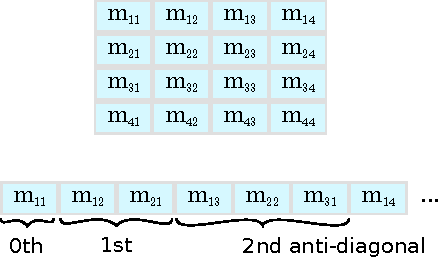
\includegraphics[scale=0.9]{figures/indexing.pdf}
  \caption{DPM memory layout}
  \label{fig:indexing}
\end{figure}

We index the matrices using a modified version of the \textit{Cantor pairing function}, where a tuple is assigned to an offset.
The original Cantor pairing function $\pi$ assigns an integer to a pair of integers (e.g., $\pi: (\mathbb{N}, \mathbb{N}) \rightarrow \mathbb{N}$).
Since the size of the DPM is given by the length of the input sequences and because it is not infinite,
we modified the pairing function to accept a tuple of two integers from the interval $[0..\textrm{length}(\textrm{Sequence 1\textbar2})]$ as input.
As a consequence, the DPM is divided into three parts: the \emph{opening}, \emph{intermediate}, and \emph{closing part}.
In the opening part, the modified pairing function is identical to the original function; in the intermediate and closing parts,
the modified pairing function is calculated by subtracting an offset from the original pairing function.
We calculate the offset via the original Cantor pairing function.

\begin{figure}[ht!]
  \centering
  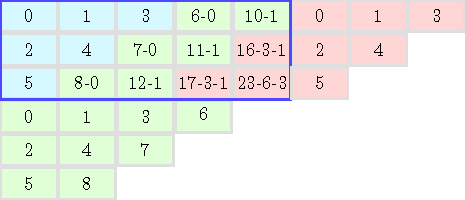
\includegraphics[scale=0.9]{figures/pairingfunc.pdf}
  \caption{Indexing scheme for anti-diagonals}
  \label{fig:pairingfunc}
\end{figure}

In Figure~\ref{fig:pairingfunc}, we show the index calculations for the anti-diagonals of a $5\times3$-matrix.
The blue frame denotes the actual boundaries of this $5\times3$ DP matrix, the blue cells represent the opening part,
the green cells inside the frame the intermediate part, and the red cells inside the frame the closing part.
Green and red cells outside the matrix boundaries represent the offset calculation for the intermediate and closing part.
For the DP calculations, only indices that correspond to DPM entries are required.
Note that, the index function has constant time and space complexity. This is essential for reducing the overhead when accessing elements in the DPMs.

Given the anti-diagonal indexing scheme for a single matrix, we can now
devise the memory layout for the three DPMs ($M^0,M^1,M^2$).
%(Nikolai) I changed the matrix names to use superscripts to keep it consistent
This is because calculating a DP value requires
accessing values from all three matrices, which are located in different
memory regions.
%Therefore, the access pattern inside the matrices follows the same anti-diagonals.
To improve data locality while, at the same time, using efficient
vector load and store operations,
the data has to be arranged accordingly.  Since we are using
double-precision floating-point numbers for all calculations, an SSE3 vector
($128$ bit) can hold 2 values, while an AVX vector ($256$ bit) can hold 4 values.
To this end, we evaluated the following three alternative matrix layouts (see Figure~\ref{fig:datalayout}), 
where \verb|n| always is the number of elements in one matrix and \verb|m = n / v| the number of vectors per matrix for vector size \verb|v|.
{\bf AS: is this correct?}
{\bf NB: No, n is the number of elements in the matrix (i.e., n = length(seq\_a) * length(seq\_b)). I corrected that in the text and added a description for m as well.}

\begin{figure}[ht!]
  \centering
  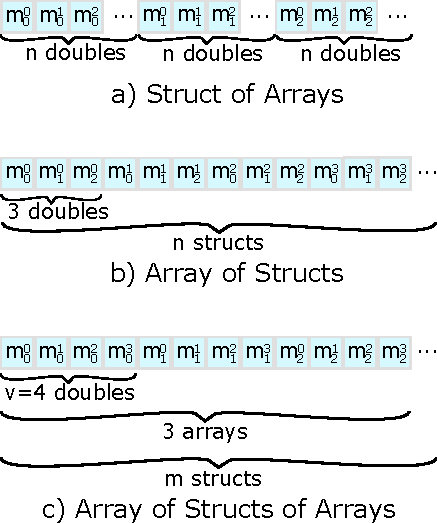
\includegraphics[scale=0.7]{figures/datalayout.pdf}
  \caption{Alternative data layouts for storing anti-diagonals}
  \label{fig:datalayout}
\end{figure}


\paragraph*{Struct of Arrays (SoA)} ({\small\texttt{struct \{ double m0[n], m1[n], m2[n]; \} data;}})
% NB: With n being introduced in the previous paragraph, we probably won't need to describe this again.}
% Here, \verb|n|, is the number of anti-diagonals.
This layout allows for simple vector load and store operations.
However, the three DPMs are located in separate memory regions, which decreases
data locality and hence cache efficiency.

\paragraph*{Array of Structs (AoS)} ({\small\texttt{struct \{ double m0, m1, m2; \}
data[n];}}) This layout exhibits improved data locality by grouping values
closely together that are -- in most cases -- accessed simultaneously. On the
other hand, loading and storing vectors requires disentangling and interleaving
them, which requires several, potentially costly, vector shuffle operations.

\begin{figure}[ht!]
  \centering
  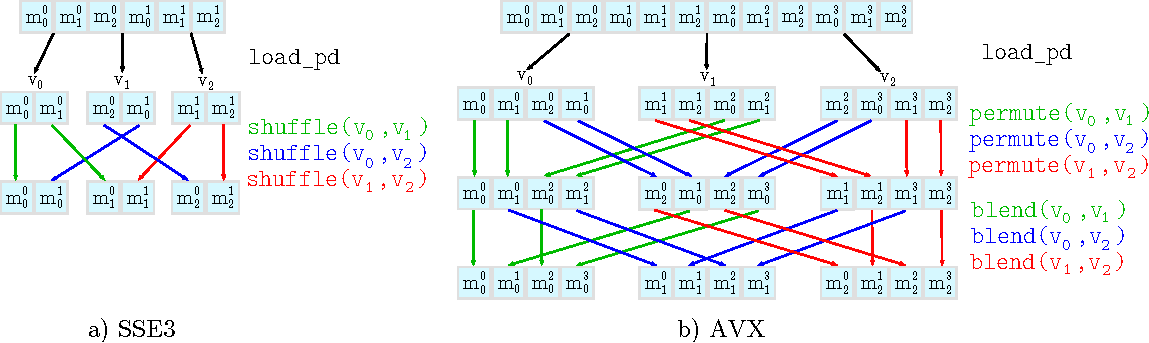
\includegraphics[scale=0.6]{figures/shuffle.pdf}
  \caption{Disentangling operations for a) SSE3 (128 bit) and b) AVX (256 bit) vectors.}
  \label{fig:shufflesse}
\end{figure}

Figure~\ref{fig:shufflesse} illustrates these shuffle operations.
For a particular position on an anti-diagonal, we use $m_x^y$ to denote that element $m$ of a DP matrix with index $x$ 
is stored in slot $y$ of the SSE3/AVX vector.
%\textbf{TF: Daniel, would the previous sentence cover what you wanted to say?}
%For $m_x^y$, the subscript $x$ indicates
%the index of the matrix and the superscript $y$ the SSE3/AVX vector element
%index $y$
%${\bf TODO (Daneil) Is it correct to repeat the $y$ at the end of the sentence? I would also insert another verb as "denotes" ...and the superscript $y$ denotes the SS3/AVX...}.
The first row of the Figure depicts the {\em AoS} data layout.
Initially, we perform a vector \texttt{load} operation
to load the data into temporary vector registers.
Thereafter, we shuffle the temporary vectors such that (i) each vector only contains elements from one of the three DP matrices and
(ii) the individual elements are in the correct order with respect to  the anti-diagonal.
For both, SSE3 as well as AVX instructions, we need to perform three \texttt{load} operations and three \texttt{shuffle}/\texttt{permute} operations.
For AVX, three additional \texttt{blend} operations are required to correctly order the data elements.

\paragraph*{Array of Structs of Arrays (AoSoA)} ({\small\texttt{struct \{ double m0[v],
m1[v], m2[v]; \} data[m];}}) This layout stores vectors such that
adjacent elements for each of the three matrices can be directly loaded into an SSE3/AVX vector. % (Nikolai) Quick typo fix
While solving both aforementioned problems (low data locality and costly vector operations),
this complicates DP cell accesses above the current anti-diagonal.
The required values above the current anti-diagonal are not stored contiguously
and therefore we either need to use \texttt{shuffle}/\texttt{permute} operations
or conduct partial loads (i.e., load single elements into vectors).

\paragraph*{} All three layouts exhibit different performance characteristics with respect to
cache efficiency and complexity of the load, store, as well as shuffle operations.
We implemented prototypes for all three approaches to analyze their
performance and found that the AoS approach performs best.
Note that, the computational cost of the \texttt{shuffle} operations outweighed the improved cache efficiency in the AoS and
AoSoA layouts (also see Table~\ref{tbl:benchmark-layout} in Section~\ref{res-team-1}).


\subsection{Memoization}
\label{ssec:memo}

The TKF91~\cite{TKF91} model
%(Nikolai) Added the model name so that the sentence would make sense without the reference.
has several parameters. Thus, it initially seemed inevitable to carry out the non-trivial computations for filling DP cells
from scratch for each individual cell.
However, after analyzing which expressions are constant and can thus be pre-computed and reused (i.e., memoized),
we reduced the operations required for calculating a DP cell value to just three: indirection, summation, maximum.

Obvious savings can be achieved for expressions that only depend on the time parameter $t$,
the birth rate $\lambda$, and the death rate $\mu$.
These values are constant and given as input parameters.
We also observed that the cell updates in the DP algorithm only require a constant number of common sub-calculations/components:
When the nucleotide states at the current indices for the two sequences are available,
the score (cell value) can be computed by only using the current nucleotide pair and the
neighboring values in the three DP matrices.

The memoization scheme (lookup table) for all possible configurations is shown in Figure~\ref{fig:memo}.
The penalty functions $C^i$ take one or two nucleotide states as parameters.
Thus, these penalties can be stored in a memoization table of $4$ and $16$ entries, respectively.
Using only $24$ memoized values, we were able to substantially simplify and accelerate the cell updates.
In addition, this simplification now allows to apply the logarithm for preventing numerical underflow.
This was not possible before, since taking the logarithm of the original equation would have been too expensive computationally.
In addition, vectorizing the cell updates is simpler, since the remaining calculations are less complex.
Finally, this simplification reduces the number of possible memory layout and vectorization options.

\begin{figure}
\[
\begin{aligned}
  C^0(a)&=\frac{\lambda}{\mu}\pi_{a}\overline{p_0}(t)\\
  C^1(a, b)&=\frac{\lambda}{\mu}\pi_{a}max\{P_{a \rightarrow b}(t) p_1(t), \pi_{b}\overline{p_1}(t)\}\\
  C^2(b)&=\pi_{b}\lambda\beta(t)\\
  M^0(i,j)&=C^0(a_i)max\{M^0(i-1, j), M^1(i-1,j), M^2(i-1,j)\}\\
  M^1(i,j)&=C^1(a_i,b_j)max\{M^0(i-1, j-1), M^1(i-1,j-1), M^2(i-1,j-1)\}\\
  M^2(i,j)&=C^2(b_j)max\{M^1(i,j-1), M^2(i,j-1)\}
\end{aligned}
\]
\caption{A re-formulation of the DP step using the memoized sub-problems (lookup tables) $C^i$.}
\label{fig:memo}
\end{figure}

At a later point of the project, it became evident that the indexed loads from the memoized penalty matrices $C^0$, $C^1$, $C^2$, as shown in Figure~\ref{fig:memo}
caused a performance degradation.
To address this problem, we tried to pre-compute a larger lookup table of vector-sized elements, that we indexed by a specific nucleotide permutation.
Consider the following example for AVX vector intrinsics.
We need to calculate a bijective mapping for a set of four nucleotides to an integer representing one of the $4^4 = 256$ possible permutations (e.g., a perfect hash)
for $C^0$ and $C^2$, and one of the possible $4^{2 \cdot 4} = 65536$ permutations for $C^1$ respectively.
The mapping is implemented as base conversion from the set of 4 nucleotides to an unsigned integer via appropriate bit operations.

While this approach has exponential space requirements as a function of the vector width, using a lookup table of $65536 \cdot 32$ bytes $= 2$ MB for $C^1$ for
the AVX version of our code was still feasible.
However, the performance evaluation revealed that too much time is spent to populate the table.
Thus, we abandoned this approach.

% AS: habe den rest mal auskommentiert hier den brauchen wir nicht wirklich
%Since the values in the table only depend on the likelihood model parameters, that is, it is independent of the input sequences at hand,
%this approach can be re-considered in cases were this lookup table shall be re-used for multiple DP invocations.
%This might be useful when calculating pair-wise alignments of $n$ sequences under the same model parameters and
%{\bf not sure if we should write this here, at leats as long as the parameter t is also required to calculate the values in that table, need to double-check}{\bf That's a good point. I was mentally pul%ling t into the model, which is incorrect, unless t stays constant. }
%{\bf I don't understand the following sentence, please re-forumulate it} {\bf Tried to clarify with the part following e.g. } The scaling to wider vector registers could be retained by loading a regist%er in packs of four values, e.g. for an 8 element vector, loading the lower and upper 4 values separately from the lookup table for 4 element vectors allows the space complexity to stay constant with r%espect to vector width.


\subsection{Vectorization}
\label{ssec:vectorization}

We implemented a vectorized version for computing
$M^0$, $M^1$, and $M^2$ using \texttt{add}, \texttt{max}, \texttt{load}, and \texttt{store}
operations for both SSE3 and AVX instructions.
With these operations, we can process $n$ matrix elements in parallel.
Depending on the location of the vector on the anti-diagonal that is being processed, there will be $0 < n \leq V$ valid elements to operate on
per vector (with vector size $V := 4$ for AVX and $V := 2$ for SSE3).

Usually, data that has to be loaded into vectors needs to be aligned, that is, the starting 
address of the vector data needs to be a multiple of 16 or 32 bytes. This memory alignment allows to
use the aligned versions of the vector \texttt{load} and \texttt{store} operations,
which are faster than the respective unaligned operations.
Although we ensured memory-aligned accesses to the majority of the data (as will be explained in
Section~\ref{ssec:dataalignment}), we consistently used unaligned vector \texttt{load} and \texttt{store}
operations (\texttt{loadu\_pd} and \texttt{storeu\_pd}) in the SSE3 and AVX versions of our code.
We did not observe a significant performance degradation when
applying unaligned load intrinsics on aligned data.

To prevent our \texttt{store} operations from overwriting data at the boundaries
of the matrices, we ensured that for vectors with size $n < V$ (i.e.,
not completely filled/padded vectors) only $n$ elements are written back into the
matrices.  For the SSE3 version, this can be achieved by only writing the lower
part of the vector if its size is $1$.  For AVX, however, we covered all cases
where $n < V$ holds using the \texttt{maskstore\_pd} intrinsic and an appropriate mask
for all possibles values of $n$ (i.e., $3$, $2$, and $1$).

\subsection{Data Alignment}
\label{ssec:dataalignment}

If we want to vectorize along the anti-diagonals, accessing the memory in the DPMs when they are stored in row-, or column-major order 
decreases efficiency. This is because such a DP storage scheme does not allow to deploy efficient vector operations for loading the values from the matrices into vector registers.
For such a matrix layout, the performance of the inner DP loop becomes heavily memory-bound.
Therefore, we used the aforementioned layout by consecutive anti-diagonals together with the struct of arrays approach (see section~\ref{ssec:memorylayout}),
such that unaligned \texttt{load} and \texttt{store} operations for moving data directly to/from the anti-diagonal
into vector registers can be utilized.

% AS: habe den paragraphen hier unten mal auskommentiert, der ist zu redundant mit der scetion drüber
%Those \texttt{load} and \texttt{store} operations come in two flavors: There exist \texttt{load} and \texttt{store} operations for aligned and unaligned data.
%Using the unaligned versions can decrease memory access performance. However,
%as mentioned in Section~\ref{ssec:vectorization}, loading aligned data using \texttt{loadu\_pd} does not incur a performance penalty.
%On the other hand, using aligned loads yields storing the DP matrices more complex.
%When loading data from the matrices into SSE3/AVX vector registers, the data has to be aligned to $16/32$ byte boundaries.

\begin{figure}[ht!]
  \centering
  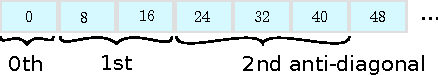
\includegraphics[scale=0.9]{figures/unaligned.pdf}
  \caption{Shift of the byte offset of the anti-diagonals}
  \label{fig:unaligned}
\end{figure}

Figure~\ref{fig:unaligned} shows why a 16/32 byte alignment for the starting addresses of the anti-diagonals can not be achieved when just
storing anti-diagonals linearly. To solve this problem, we used padding, that is, we allocate some dummy entries such that
each anti-diagonal starts at a 16/32 byte-aligned address.
As a consequence we also had to modify the indexing function from Section~\ref{ssec:memorylayout} accordingly.
The main idea is to store each anti-diagonal starting at a 16/32 byte-aligned address.

%AS habe das unten mal auskommentiert
%Thereby, all load and store operations are guaranteed to happen on a predictable alignment, which we choose so that most of the operations happened on a proper alignment boundary.
%When iterating over anti-diagonal elements in a vectorized fashion, the vectors are then automatically constructed from data that is aligned to the required address offset.

%{\bf The following three sentences need to be re-written, they are rather confusing}
%{\bf I rewrote them. Is it clearer now?}

We implemented a scheme where the row with index $1$ is memory-aligned, because the row with index $0$ is initialized {\em prior} to entering the DP loop.
As a consequence, each anti-diagonal is aligned to an ``odd'' address ($a - 8$, where $a$ is the desired byte alignment, for instance, $32 - 8 = 24$ bytes for AVX intrinsics).

%The starting address for the anti-diagonal is not the required alignment address for loading and storing the vectors, but a larger address minus the size of one double floating point value.
%This is due to the fact that the row with index 0 of the matrix is pre-computed during the matrix initialization and therefore a value is never written to this row. Another reason for this decision is that it is impossible to load all vectors needed for the computation inside the tight loop of the algorithm from an aligned addresses.

\begin{figure}[ht!]
  \centering
  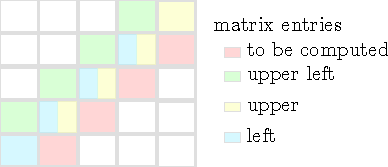
\includegraphics[scale=1.1]{figures/alignment.pdf} \caption{Outline of the
  data accesses required for calculating an anti-diagonal.\textbf{TF: I think
  the diagram is rather confusing. Why not just draw a grayscale matrix with
  arrows originating from the red cells to indicate dependencies? }}
  \label{fig:alignment}
\end{figure}

In Figure~\ref{fig:alignment}, we show a snapshot of the required values for computing the anti-diagonal elements with AVX intrinsics (vector length: $4$ double precision values).
In the current step we want to calculate the red elements.
For calculating a single element, we require three elements from the two previous anti-diagonals.
We need to access the element directly above (yellow) and left (blue) to the current element as well as the diagonal element above and to the left  (green).
The Figure illustrates that ---omitting the asymptotically irrelevant boundary cases--- one of the following four conditions holds:
\begin{enumerate}
  \item red and blue start on an aligned address, yellow and green do not
  \item red and yellow start on an aligned address, blue and green do not
  \item yellow and green start on an aligned address, red and blue do not
  \item red and green start on an aligned address, yellow and blue do not
\end{enumerate}

For the computation, we need to perform three \texttt{load} operations in total for the blue, yellow, and green elements as well as one \texttt{store} operation for the red elements.
Since, based on empirical observations, {\em unaligned} \texttt{store} operations require more time than {\em unaligned} \texttt{load} operations,
we ensured that either condition $1$ or $2$ above is always met.
Thus, we implemented our code such that, the first condition is met for the opening and intermediate part and the second condition holds true for the closing part of the DP matrices.

%We achieved an appropriate memory-alignment for each anti-diagonal by padding them as needed.

% I think we don't need the stuff below.
%We realized this padding by modifying the indexing function into the matrices. In the final version of this indexing function for an anti-diagonal, a certain amount of array elements in the matrix buffer is skipped. Elements are skipped until the second element of the anti-diagonal is aligned with the vector intrinsics requirements. This way, some memory is wasted because it is not used, however it is asymptotically insignificant compared to the overall space complexity of the algorithm ($O(\textrm{length}(\textrm{Sequence 1}) \cdot \textrm{length}(\textrm{Sequence 2}))$).

\section{Implementation of Team II}
\label{sec:implementation-2}

In the following, we first describe how we transformed the algorithm into log-space to prevent numerical underflow.
This also allowed us to simplify the formulas.
Thereafter, we report how we improved data locality by storing the matrix entries in a dedicated data structure.
While we experimented with different vectorization techniques, it turned out that the fastest code did not rely on vectorization.
We conclude, that we managed to simplify the sequential code to a point, where the vectorization overhead (see Section~\ref{sec:vector}) 
exceeds the performance gains that can be achieved.

\subsection{Mathematical Optimization - Basic Version}

\subsubsection{Numerical Underflow Prevention}
\label{sec:log}

As the TKF91 algorithm performs successive multiplications of floating point numbers, preventing numerical underflow
{\em is} a major issue. Underflow can occur, even for short input sequences with less than $100$ nucleotides each.
To address this issue we transformed all computations into log-space, to add logarithms of probabilities instead of multiplying probabilities.
While it is still possible to experience numerical underflow, even after this transformation,
we expect that this is highly unlikely to occur for practical (empirical) input data.
We did not observe any numerical underflow for the range of input parameter values and sequence lengths (up to and including $10,000$ nucleotides)
we tested. 

\subsubsection{Simplifying the Formulas}
We were able to omit redundant computations by re-using already computed values from previous matrix entries.
For example, we observed that $$M^0(i+1,0) = M^0(i,0) + \log(\gamma_{i+1}) + \log(\zeta_{i+1}) + \log(\beta(t)) + \log(\pi_{a_{i+1}}) + \log(\bar{p_0}(t)).$$
After replacing $\beta(t), \bar{p_0}(t), \gamma_i$, and $\zeta_i$ by their respective formulas, we noted that some terms appear multiple times.
Operating in log-space allowed us to further simplify the formulas. Especially the logarithmic rules $\log(a*b) = \log(a) + \log(b)$ and $\log(a/b) = \log(a) - \log(b)$
allowed us to replace multiplications and divisions with additions and subtractions.

In the following formulas, $1 \leq i \leq n$ and $1 \leq j \leq m$, if not stated otherwise.

\paragraph{Matrix Initialization}
\label{sec:formulas:init}
\begin{align*}
M^0(0,0) &= -\infty \\
M^1(0,0) &= \log(\gamma_0) + \log(\zeta_1)
		= \log(1-\frac{\lambda}{\mu}) + \log (1 - \lambda * \beta) \\
M^2(0,0) &= -\infty \\
M^0(1,0) &= \log(\gamma_1) + \log(\zeta_1) + \log(\bar{p_0}) + \log(\pi_{a_1}) \\
		&= \log(1- \frac{\lambda}{\mu}) + \log(\lambda) + \log(1- \lambda *\beta) + \log(\beta) + \log(\pi_{a_1}) \\
M^0(i,0) &= M^0(i-1,0) + 2*\log(\lambda) + 2*\log(\beta) + \log(\pi_{a_i}), i \geq 2 \\
M^1(i,0) &= -\infty \\
M^2(i,0) &= -\infty \\
M^0(0,j) &= -\infty \\
M^1(0,j) &= -\infty \\
M^2(0,1) &= \log(\gamma_0) + \log(\zeta_2) + \log(\pi_{b_1}) \\
		&= \log(1- \frac{\lambda}{\mu}) + \log(1-\lambda*\beta) + \log(\lambda) + \log(\beta) + \log(\pi_{b_1}) \\
M^2(0,j) &= M^2(0, j-1) + \log(\lambda) + \log(\beta) + \log(\pi_{b_j}), j \geq 2 \\
\end{align*}


\paragraph{Further Initialization}
\label{sec:formulas:further}
\begin{align*}
M^0(i,j) &= \log(\lambda) + \log(\beta) + \log(\pi_{a_i}) \\
M^1(i,j) &= \log(\lambda) - \log(\mu) + \log(\pi_{a_i}) + \log(\max\{P_{a_i \to b_j} * \bar{p_1}, \pi_{b_j} * \bar{p_1}\}) \\
	&= \log(\lambda) - \log(\mu) + \log(\pi_{a_i}) + \log(1-\lambda * \beta) + \max \begin{cases}
	\log(P_{a_i \to b_j}) - \mu*t, \\
	\log(\pi_{b_j}) + \log(1- e^{- \mu*t} - \mu * \beta)
\end{cases} \\
M^2(i,j) &= \log(\lambda) + \log(\beta) + \log(\pi_{b_j})
\end{align*}

\paragraph{Dynamic Programming Step}
\begin{align*}
M^0(i,j) &= M^0(i,j) + \max\{M^0(i-1,j), M^1(i-1,j), M^2(i-1,j)\} \\
M^1(i,j) &= M^1(i,j) + \max\{M^0(i-1,j-1), M^1(i-1,j-1), M^2(i-1,j-1)\} \\
M^2(i,j) &= M^2(i,j) + \max\{M^1(i,j-1), M^2(i,j-1)\}
\end{align*}

\subsubsection{Pre-computing the Logarithms}
In general, replacing a multiplication by two logarithms and an addition is more costly.
However, we managed to circumvent the additional computational cost of log space.
This is because our formulas above contain only $25$ different logarithm invocations that only depend on given, constant input parameters.
Hence, all these logarithms can be pre-computed.

A major disadvantage of logarithmic transformations is that errors in the logarithm computation accumulate over a sequence of operations.
To further investigate this, we used the high precision mathematical library of the \texttt{boost}-framework \cite{boost}.
It offers datatypes that dynamically adapt their floating point precision to avoid numerical errors as well as under-/overflow.
Our initial idea was to use this library only for pre-computing the logarithms, and thereby reduce the induced runtime overhead.
However, converting these arbitrary precision datatypes back into standard double precision floating point values
introduced additional loss of precision {\bf AS: with respect to the standard log function?},
when applying the respective conversion functions {\bf AS: please name the conversion functions you used!}.
Therefore, we abandoned this path.

In the rest of the manuscript we refer to the code obtained by applying the above techniques and transformations as the basic version.

\subsection{Matrix Storage Schemes - Improved Version}
\label{sec:caching}

\subsubsection{Matrix as Array}
In the first, na\"ive implementation, we stored each matrix ($M^0, M^1$, $M^2$) in a separate array, using row-major order.
The matrix entry at position $(i,j)$ is stored at index position $i*(m+1)+j$ in the array (see Figure~\ref{fig:rowmajor}).


\begin{figure}
\begin{minipage}{0.7\textwidth}
\centering
\begin{tabular}{|c|c|c|c|c|}
\hline
0 & 1 & 2 & 3 & 4 \\
\hline
5 & 6 & 7 & 8 & 9 \\
\hline
10 & 11 & 12 & 13 & 14 \\
\hline
15 & 16 & 17 & 18 & 19 \\
\hline
\end{tabular}
\caption{Row-major indexing}
\label{fig:rowmajor}
\end{minipage}
\end{figure}

To illustrate the shortcomings of this approach, consider the following example: assume that six matrix rows fit into one cache line.
Then, performing one iteration of the inner DP loop requires loading three cache lines, one per DPM.
This is depicted in part a) of Figure~\ref{fig:cachelines}.
If we further assume a cache capacity of only two cache lines,
every iteration would then force one of the lines to be swapped out and decrease memory efficiency.

\begin{figure}
\centering
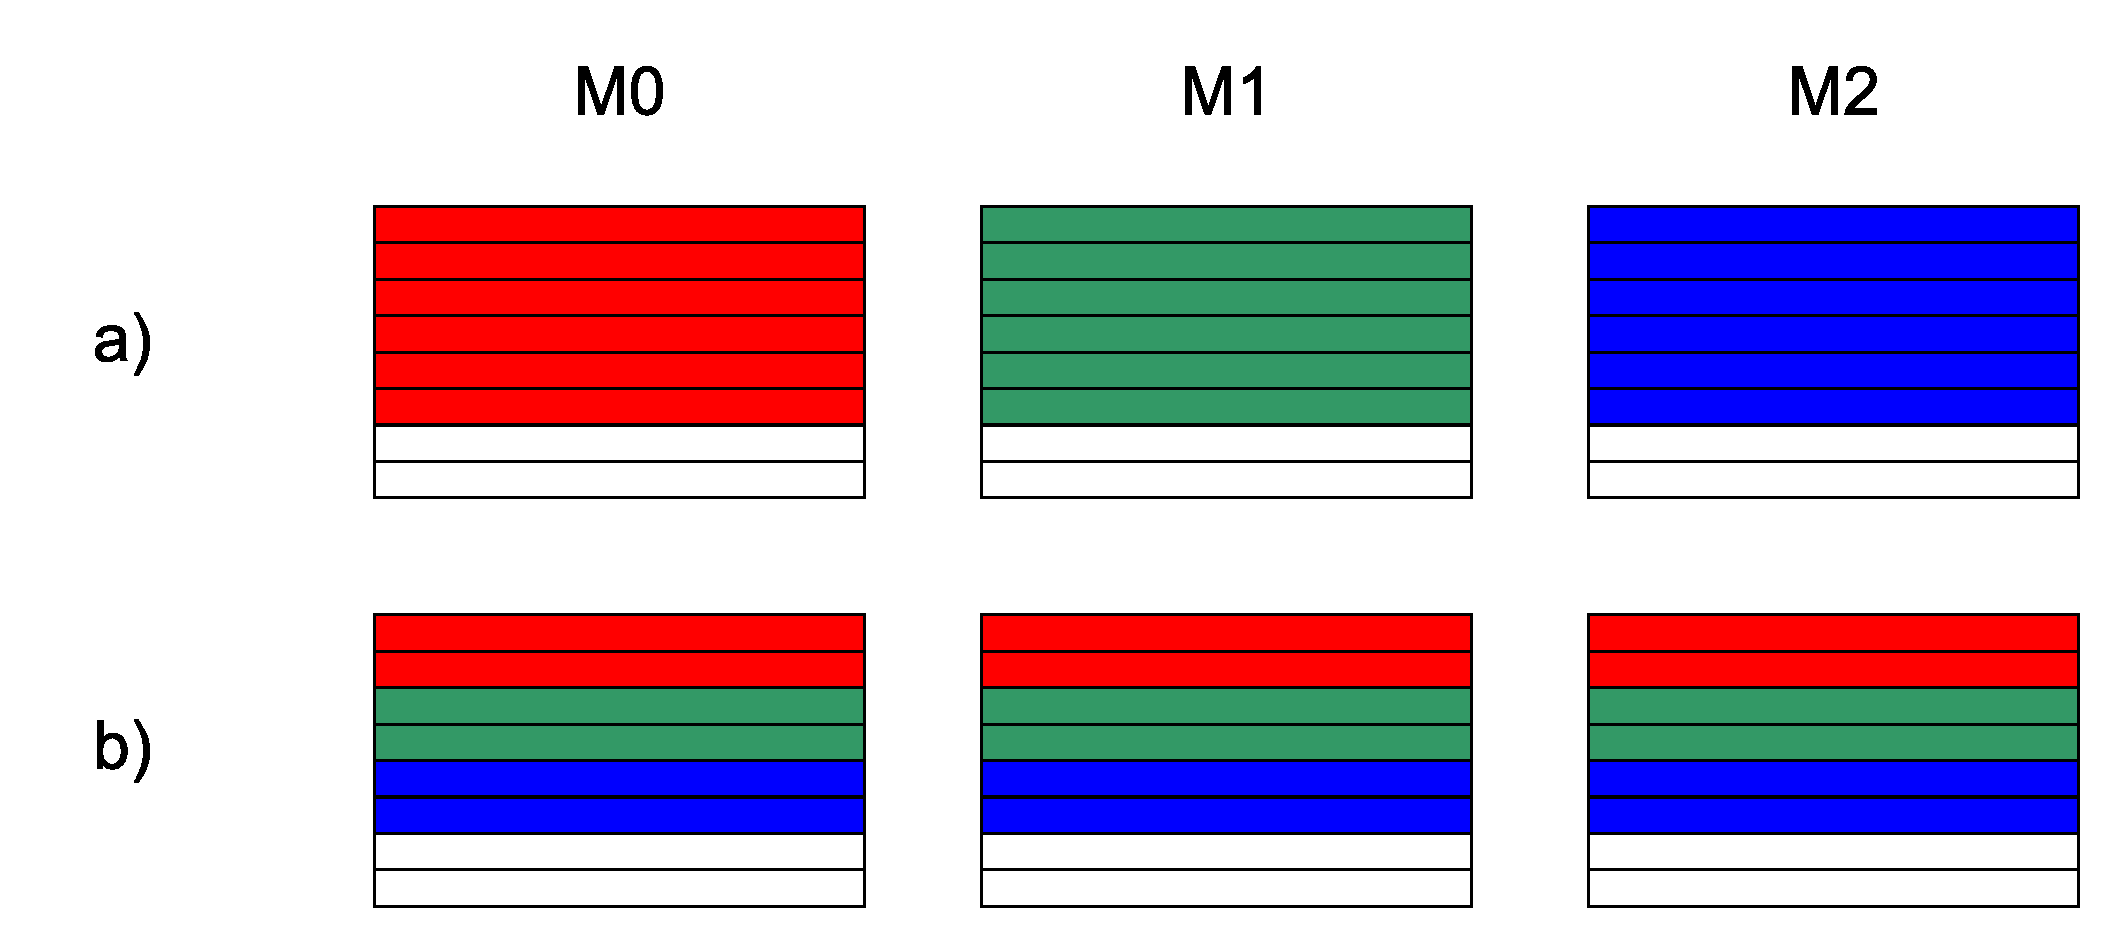
\includegraphics[width=\textwidth]{images/cachelines.pdf}
\caption{Relation of cache lines and matrices, using the method of allocating each matrix separately(\textbf{a)} and the Array-of-Structs method (\textbf{b)}.
Each color represents a distinct cache line.}
\label{fig:cachelines}
\end{figure}

\subsubsection{Array-of-Structs Data Structure}
The dynamic programming step (see Algorithm~\ref{alg:dp}) accesses the matrices $M^0, M^1$ and $M^2$ at the same index position to determine the maximum entry.
Thus, we improved data locality by storing the entries from the three matrices located at identical index positions contiguously in memory.
For this, we implemented a data structure called \texttt{MatrixEntry} that consists of three double values: \texttt{$m_0$}, \texttt{$m_1$} and \texttt{$m_2$}.
Then, we used the Matrix as Array approach as before, but containing \texttt{MatrixEntry} structs as elements instead of simple
\texttt{double} values (see Figure~\ref{fig:aos}). 
\textbf{TF: The sentence is not very clear and must be re-written or re-formulated. 
The term Matrix as Array is not defined. Did you have SoA or AoS in mind?}

Let us now consider the example in Figure~\ref{fig:cachelines} again.
With six matrix lines filling one cache line, a cache line now contains data from all three matrices.
Consequently, all operations for a single DP cell update
will access at most two cache lines.
If we assume a cache capacity of two cache lines again, cache misses will now only occur when traversing row boundaries.

By using the \texttt{perf stat} tool, we found that using the \texttt{MatrixEntry} data structure indeed reduced
the number of page faults which we use as a proxy for cache efficiency.
{\bf AS: why didn't you use cachegrind then if perf-stat yielded variable results and only reprts page faults?}


\begin{algorithm}

\ldots\tcp{some initializations, see Appendix~\ref{sec:formulas:init}}
\For{$i = 1 , \ldots, n$} {
	\For{$j = 1, \ldots, m$} {
		\ldots\tcp{some initializations, see Appendix~\ref{sec:formulas:further}}

		$coord \gets CO(i, j)$\;
		$up \gets CO(i, j-1)$\;
		$diag \gets CO(i-1, j-1)$\;
		$left \gets CO(i-1, j)$\;

		$m[coord].m_0 \gets m[coord].m_0 + \max\{m[left].m_0, m[left].m_1, m[left].m_2\}$\;

		$m[coord].m_1 \gets m[coord].m_1 + \max\{m[diag].m_0, m[diag].m_1, m[diag].m_2\}$\;

		$m[coord].m_2 \gets m[coord].m_2 + \max\{m[up].m_1, m[up].m_2\}$\;
	}
}

\caption{The dynamic programming step, row-major version}
\label{alg:dp}
\end{algorithm}

\begin{figure}[width=\textwidth]
\centering
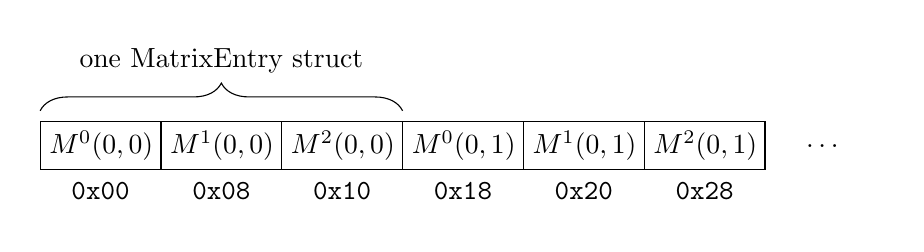
\begin{tikzpicture}[
    every node/.style={align=center, minimum height=1.5em, minimum width=1.5cm,node distance=0pt},
    background rectangle/.style={fill=black!0},show background rectangle,
    ]
\node [cell](n1) at (0,0) {$M^0(0,0)$};
\node [cell, right = of n1] (n2) {$M^1(0,0)$};
\node [cell, right = of n2] (n3) {$M^2(0,0)$};
\node [cell, right = of n3] (n4) {$M^0(0,1)$};
\node [cell, right = of n4] (n5) {$M^1(0,1)$};
\node [cell, right = of n5] (n6) {$M^2(0,1)$};
\node [right = of n6](n7){\dots};
%\node [cell,right = of n7]{$M^2(n,m)$};

\node [below = of n1]{\texttt{0x00}};
\node [below = of n2]{\texttt{0x08}};
\node [below = of n3]{\texttt{0x10}};
\node [below = of n4]{\texttt{0x18}};
\node [below = of n5]{\texttt{0x20}};
\node [below = of n6]{\texttt{0x28}};

\draw[
   decorate,
  decoration={brace,amplitude=10pt}
]
  ([yshift=4pt]n1.north west) --
  node [black,yshift=18pt] {one MatrixEntry struct}
  ([yshift=4pt]n3.north east) ;

\end{tikzpicture}
\caption{Array-of-Structs data structure for storing the three matrices in memory. Each \texttt{MatrixEntry} element stores
the entries of a single index for all three matrices. The structs are stored contiguously in row-major order.}
\label{fig:aos}
\end{figure}

\textbf{TF: The term CO in Algorithm 1 should be defined in the manuscript at least, e.g. what it does and what it stands for}

\subsubsection{Alternative Storage Schemes}
\label{par:otherattempts}

Since each DP cell update needs to access the top, left, and upper-diagonal elements of the matrices,
storing the matrix anti-diagonals linearly (see Figure~\ref{fig:wavefront} and considerations by Team I)
will minimize cache misses.
Finding an inexpensive-to-compute closed formula that maps the index position $(i,j)$ representing the row and column of a matrix
to wave-front-coordinates turned out to be challenging (see also discussion by Team I in Section~\ref{ssec:memorylayout}).
The index of the diagonal is $i+j$, the sum of the row index and the column index.
Determining the number of elements on the anti-diagonal and especially the correct position along the anti-diagonal proved more difficult though.
The indexing formulas we tested were too computationally expensive and required more computations than the actual cell updates.
As an alternative, we tried storing pre-computed index mappings in an additional matrix.
However, this slowed down the program as computing the mapped indices required more arithmetic operations than the actual TKF91 algorithm.
Figure~\ref{fig:offset} illustrates the main problem which has to be solved
for efficiently indexing-diagonals: Given an wave-front index $k$, how do we obtain the indices for the upper, upper-left-diagonal, and left element of the matrix?
While the required offsets are constant for a single anti-diagonal, they change for successive anti-diagonals.



\begin{figure}
\begin{minipage}{0.5\textwidth}
\centering
\begin{tabular}{|c|c|c|c|c|}
\hline
0 & 1 & 3 & 6 & 10 \\
\hline
2 & 4 & 7 & 11 & 14 \\
\hline
5 & 8 & 12 & 15 & 17 \\
\hline
9 & 13 & 16 & 18 & 19 \\
\hline
\end{tabular}
\caption{Wave-front indexing}
\label{fig:wavefront}
\end{minipage}
\end{figure}

\begin{figure}
\centering
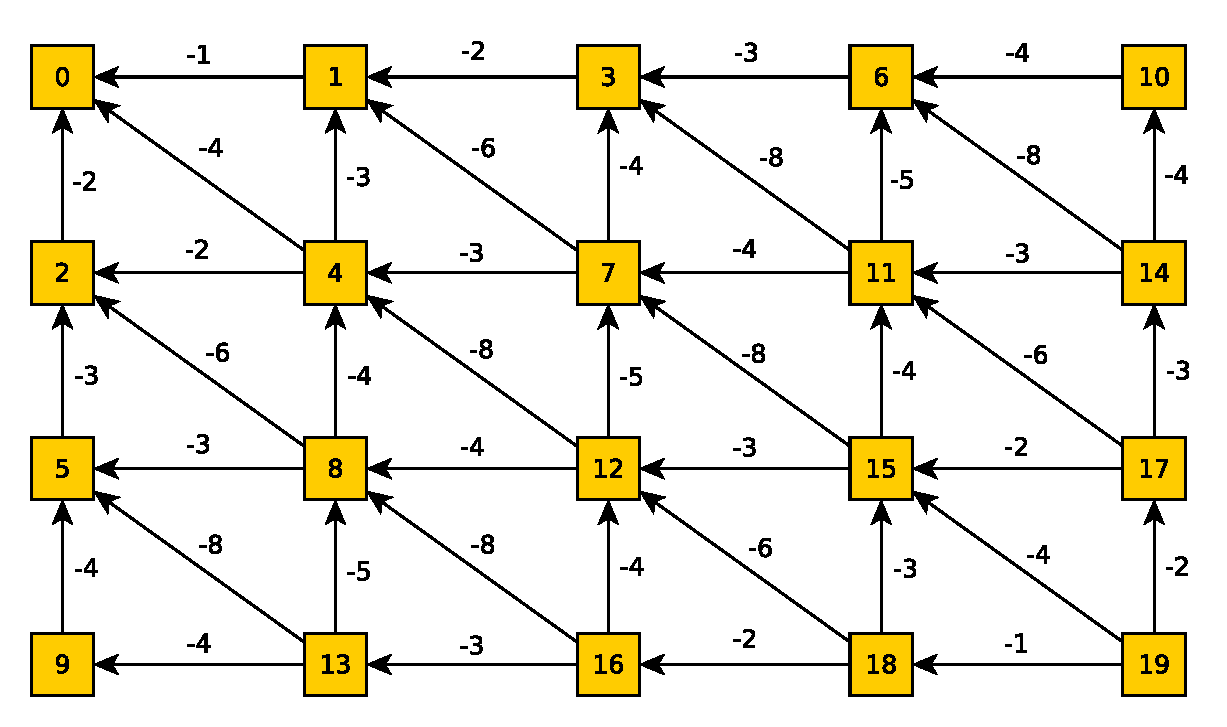
\includegraphics[scale=0.5]{images/unnamed0.pdf}
\caption{Offsets in wave-front/anti-diagonal indexing}
\label{fig:offset}
\end{figure}

%\section{Further Performance Tuning}
%- crlibm library
%- fixed-size array, no memset
%- store sequences as array of integers, used as a fast way to index precomputed logarithm values
%- fill matrices simultaneously (in the same loop)

We denote the code obtained by applying the above storage scheme, the improved version.

\subsection{Vectorization Attempts}
\label{sec:vector}
During code development we conducted a partial vectorization for two of our implementations:
the basic log-space implementation (Section~\ref{sec:log}) and the improved log-space implementation, using a more
cache-efficient data structure to store the matrices (Section~\ref{sec:caching}).

In both cases we mainly focused on vectorizing the code that initializes the three matrices.
This is because our analyses with \texttt{Valgrind callgrind} revealed, that this
part of the code required $75-80\%$ of overall runtime.
Additionally, as the initializations are completely independent of each other, this part should be straight-forward to vectorize.

Several code transformations were necessary to vectorize the code.
First, we had to ensure that vector \texttt{load} and \texttt{store} operations are performed on correctly aligned memory addresses (see discussion by Team I).
Secondly, we needed to devise a strategy for iterating over matrices and handling matrix sizes that are not multiples of the vector width.
Finally, we needed to store calculation terms (e.g., $\log(\pi)$'s or $P_{a_i \to b_j}$'s), in appropriate vector types and
had to replace all basic arithmetic operations by their vectorized counterparts.

\subsubsection{Log-space implementation}
For the vectorization of our basic version (see Section~\ref{sec:log}), we implemented an appropriate memory alignment
by using the \texttt{\_\_attribute\_\_(aligned(\texttt{size}))} attribute for stack allocations,
and the \texttt{posix\_memalign} function for heap allocations.

We also changed the iterations through the matrices to start at entry $0$ of each row, as starting iterations at position $1$
would result in memory accesses at incorrectly aligned addresses.
Furthermore, as we store the matrix rows contiguously in memory,
we had to pad the rows to ensure a correct alignment of the first entry in each row.

The strategy we chose to deal with row dimensions that are not multiples of the vector width is straight-forward.
For each row, we compute as much as possible via vector intrinsics and the remainder sequentially.

\subsubsection{Version using Array of Structs data structure}
While the strategy for dealing with row dimensions that do not fit vector widths remained the same in the improved version (introduced in Section~\ref{sec:caching}) of our program,
we had to apply several modifications to be able to use vector intrinsics in conjunction with this more cache-efficient data structure.

As Figure~\ref{fig:aos} shows, using the Array-of-Structs scheme results in a non-contiguous storage of row entries.
As a consequence, loading and storing vector registers is not straight-forward.
To this end, we implemented load and store operations that fit our data structure.
These operations rely on vector functions that load and store single double precision floating point values.
An advantage of this is that we do not need to enforce correct data alignment any more.
However, a single  \texttt{\_mm\_load\_pd} on contiguous memory is substantially faster than a series of \texttt{\_mm\_loadl\_pd} and \texttt{\_mm\_loadh\_pd} operations
on non-contiguous memory locations using SSE3 intrinsics. 

\subsubsection{Thoughts on wave-front vectorization}
%AS: habe das auskommentiert, ist zu redundant mit TEAM-I
%{\bf Maybe somehow make the wavefront parts more consistent to avoid redundnacies?}
%As the dynamic programming step of the TKF91 algorithm has data dependencies to the cells left of, above and diagonally left above of the cell to be computed,
%parallelization/vectorization requires a \textit{wave-front} approach.

%In a wave-front parallelization scheme, matrix entries are not computed by row or by column, but rather by computing the entries of each \textit{anti-diagonal} in parallel.
%Crucially, the individual anti-diagonals have to be computed sequentially and in-order when dependencies exist between subsequent anti-diagonals.
%In this case, the current anti-diagonal is the front of the wave traversing the DP matrix.

Our two log-space versions of TKF91 reduce the DP cell update calculations that determine the largest of two or three values.
In turn, this means that the relative amount of time spent for DP cell updates is almost negligible.
Nevertheless, we invested time to explore potential vectorized wave-front versions of the program.

Initially, as Team I, we investigated appropriate DP cell storage and access schemes,
to store the data contiguously with respect to the wave-front parallelization data access pattern.
We found that, indexing a cell required 20-30 arithmetic operations as opposed to only 2-3 for the actual cell update.
Thus, merely indexing a cell, using the standard row and column coordinates, requires an excessive amount of computations.
Our preliminary benchmarks yielded absolutely no performance improvement for the vectorized versions of
the basic as well as the improved versions of our code.
Therefore, we abandoned the vectorized wave-front approach.


\section{Evaluation and Testing}
\label{sec:evaluation}

We initially describe the benchmark data we used (Section~\ref{ssec:benchmark}) as well as the experimental setup.
Then we present the runtime results for teams I and II. We conclude with a thorough analysis of the impact of the logarithm implementation used
in Section~\ref{sec:crlibm}.

%{\bf the perf results of team 1 and team 2, need to be completely re-written! AS will do the re-writing once he has the data. the logarithm section is fine}.

\subsection{Test Data and Experimental Setup}
\label{ssec:benchmark}

%An automated test suite is extremely valuable for re-factoring and optimizing the code, in that it provides the confidence of being able to detect regressions early and get helpful hints on how to fix them. We used the \textit{ctest} module of \textit{CMake} to invoke a Python script driving our console wrapper through a number of inputs. As we also used a continuous integration service running the tests on new commits, we could easily spot when a change accidentally broke the build. This development process lead to a high level of satisfaction and faith to try out different ideas in separate branches, while immediately getting feedback.

%{\bf TODO consistency}

For testing and performance assessment, we used empirical benchmark datasets. We download multiple sequence alignments (MSAs) from \url{http://goo.gl/nlD4nb}
that were used in~\cite{bininda2005transalign}.
From each of the six MSAs, we selected ten sequences (e.g., for an MSA with $60$ sequences we extracted the sequences with indices $0, 6, 12, ..., 54$),
and initially disaligned the sequences (removed all MSA gaps).
Then, we computed all $45$ pairwise TKF91 alignments between
these ten sequences. As input parameter values, we used $\lambda:=1.0, \mu:=2.0, \tau:=0.1, \pi:=(0.27, 0.24, 0.26, 0.23)$.
We empirically determined that using median of five samples, where each sample corresponds to 
the average runtime for ten TKF91 executions (i.e., a total of $5*10*45 = 2250$ pair-wise TKF91 alignments per dataset)
yielded stable runtime estimates.

%{\bf TODO: so these were multiple sequence alignments, how did you transform them/use them to test pair-wise alignment of unaligned sequenes?}
%{\bf (Sebastian) Covering that part in the next subsection, feel free to move it. }

As test platform we used the aforementioned reference hardware (see Section~\ref{setup}).

In Sections~\ref{res-team-1} and~\ref{res-team-2} the two student teams present results of specific performance and accuracy issues they investigated in detail.
In Section~\ref{team-contest} we compare the runtimes of the implementations developed by teams I and II.

\subsection{Results of Team I}
\label{res-team-1}


As mentioned in Section~\ref{ssec:dataalignment}, we performed various performance tests using this benchmark suite.
We tested different vector load/store schemes and measured the run times of the SoA, AoS, and AoSoA storage schemes.
We show the results of the SoA versus AoS versus AoSoA runtime experiments in Table~\ref{tbl:benchmark-layout}.
As already mentioned in Section~\ref{ssec:dataalignment}, the SoA approach performs best.



\begin{table}[]
\centering
\label{tbl:benchmark-layout}
\begin{tabular}{llll}
\begin{tabular}[c]{@{}l@{}}ms per iteration\\ (compared to best)\end{tabular} & SoA                & AoS                & AoSoA        \\
BDNF                                                                                      & 83.1 (1.01)        & {\bf 82.2 (1.00)}  & 85.1 (1.04)  \\
cytb                                                                                      & {\bf 262.9 (1.00)} & 290.7 (1.11)       & 296.5 (1.13) \\
RAG1                                                                                      & 209.1 (1.02)       & {\bf 205.6 (1.00)} & 209.4 (1.02) \\
RAG2                                                                                      & {\bf 246.1 (1.00)} & 250.9 (1.02)       & 258.3 (1.05) \\
RBP3                                                                                      & {\bf 346.9 (1.00)} & 363.5 (1.05)       & 376.2 (1.08) \\
vWF                                                                                       & {\bf 439.6 (1.00)} & 441.0 (1.00)       & 462.7 (1.05)
\end{tabular}
\caption{Benchmark results for the SoA, AoS, and AoSoA storage schemes.}
\end{table}

\subsection{Results of Team II}
\label{res-team-2}
We first assess the performance and impact on the output of distinct logarithm implementations (Section~\ref{sec:crlibm}).
Thereafter, we measure the runtime of our code in Section~\ref{team2-runtimes}.

%We conducted all measurements on a desktop machine with $16$ GB RAM
%a Intel\texttrademark~i7-2600 CPU with $4$ physical cores and hyper-threading.

\subsubsection{Different Logarithm Libraries}
\label{sec:crlibm}

In addition to the standard \texttt{log} function (from C++ \texttt{<math.h>}),
we also used the \texttt{crlibm} library by Daramy {\em et al.}~\cite{Daramy04}.
It includes versions of the logarithm function, which allow to explicitly specify the rounding strategy, (e.g., rounding up, rounding down, towards zero, or towards the nearest integer), to be used.

To assess the numerical stability of our alignments,  we computed the edit distances between alignments calculated using distinct logarithm implementations 
to a reference alignment using the \texttt{Boost.Multiprecision} library.
The edit distance quantifies the difference between two strings. It calculates the minimum cost sequence of string edit operations required 
(insertions, deletions, and substitutions; note that these are string edit operations not related with the TKF91 model), 
to transform one string into the other. We assigned a cost of $1$ to insertions, deletions, and substitutions of single letters.
For our tests, we aligned all possible pairs of sequences from the BDNF MSA in the aforementioned benchmark data (see Section~\ref{ssec:benchmark}).

For the alignments, we used $\lambda:=1, \mu:=2, \pi:= (0.27, 0.24, 0.26, 0.23)$ and $\tau := 0.1$.

{\bf TODO: following paragraph need to be discussed on Firday!}
In particular the \texttt{log\_ru} function from the \texttt{crlibm} library, which explicitly rounds up, produces a notably different alignment compared to
\texttt{Boost.Multiprecision} reference alignment (see Table~\ref{fig:dist}).
However, the computed likelihood scores were highly similar and the differences in the alignments were minimal {\bf between what and what?}{\bf SL: Tried to fix that. I still think it was pretty clear from the context as it was before.} between the version using \texttt{crlibm} and the version using \texttt{Boost.Multiprecision} as can be seen in Figure~\ref{fig:alignments}.
We finally decided to use the \texttt{log\_ru} function from the \texttt{crlibm} library because it yielded the same results as the reference {\bf need to explain what we mean by reference impl} 
implementation
(\url{http://sco.h-its.org/exelixis/web/teaching/practical15/scaledCode/tkf91_scaling.tar.gz}) in most cases. {\bf SL: I thought we had chosen it because it was slightly faster than the other versions and Alexis recommended the use of crlibm instead of the standard $\log$ function?}

\begin{table}[h!]

\centering

\begin{tabular}{|c|c|}
\hline
Logarithm Function & Average Edit Distance to Reference Alignment\\
\hline
\texttt{log} from \texttt{<math.h>} & 2.15 \\
\hline
\texttt{log\_ru} from \texttt{crlibm} & 33.15 \\
\hline
\end{tabular}
\caption{Average edit distances from the \texttt{Boost.Multiprecision} reference alignment for different logarithm implementations.}
\label{fig:dist}
\end{table}


\begin{figure}

\textbf{Alignment using standard C++ header \texttt{<math.h>}}
~
\\
\texttt{ACGACTAGTCA-GC-TACG-AT-CGA-CT-C-ATTCAACTGACTGACA-TCGACTTA} \\
\texttt{A-GAG-AGTAATGCATACGCATGC-ATCTGCTATT\textcolor{red}{\underline{---C}}TG-CTG-CAGTGG--T-A}
\\~\\
\textbf{Alignment using \texttt{Boost.Multiprecision}}
~
\\
\texttt{ACGACTAGTCA-GC-TACG-AT-CGA-CT-C-ATTCAACTGACTGACA-TCGACTTA} \\
\texttt{A-GAG-AGTAATGCATACGCATGC-ATCTGCTATT\textcolor{red}{\underline{---C}}TG-CTG-CAGTGG--T-A}
\\~\\
\textbf{Alignment using \texttt{log\_ru}}
~
\\
\texttt{ACGACTAGTCA-GC-TACG-AT-CGA-CT-C-ATTCAACTGACTGACA-TCGACTTA} \\
\texttt{A-GAG-AGTAATGCATACGCATGC-ATCTGCTATT\textcolor{red}{\underline{C---}}TG-CTG-CAGTGG--T-A}
\\~\\
\textbf{Alignment from reference implementation}
~
\\
\texttt{ACGACTAGTCA-GC-TACG-AT-CGA-CT-C-ATTCAACTGACTGACA-TCGACTTA} \\
\texttt{A-GAG-AGTAATGCATACGCATGC-ATCTGCTATT\textcolor{red}{\underline{C---}}TG-CTG-CAGTGG--T-A}

\caption{Numerical alignment differences for input parameters $\pi:=(0.25,0.25,0.25,0.25), \lambda:=1, \mu:= 2, \tau := 0.1$}
\label{fig:alignments}
\end{figure}

\subsubsection{Runtime Measurements}
\label{team2-runtimes}

For measuring runtimes druing code development, we used four pairs of randomly generated sequences consisting of $10$, $100$, $1000$, and $10000$ nucleotides, respectively.
%The sequences did not contain ambiguous characters.

We measured the execution times around the kernel of the program, that is, excluding any I/O required to load parameters and input sequences, or the output of the program. 
The allocation and initialization of the three DPMs form part of the kernel and were teherfore included in our measurements.
We executed the kernel multiple times for each dataset and subsequently averaged the runtimes.
To balance accuracy and overall benchmark time (see Table~\ref{fig:runs}) we used disitinct numbers of kernel invocations, depending on the dataset size.

\begin{table}
\centering

\begin{tabular}{|c|c|}
\hline
Length of Sequences & Number of Runs \\
\hline
$10$ & $10000$ \\
\hline
$100$ & $1000$ \\
\hline
$1000$ & $100$ \\
\hline
$10000$ & $10$ \\
\hline
\end{tabular}
\caption{Number of runs per sequence length}
\label{fig:runs}
\end{table}

\subsection{Performance: Team I versus Team II}
\label{team-contest}

{\bf AS: TODO teams I and II, please include example command lines for these tests!} 

{\bf NB: The Celero benchmark suite doesn't call the implementation from the
  command line. Instead, the TKF functions are called and the time is measured.
  See \url{https://github.com/sgraf812/bioinf2015/blob/master/implementation-team1/tests/benchmark.cpp#L122-L124}
  and \url{https://github.com/sgraf812/bioinf2015/blob/master/implementation-team2/tests/benchmark.cpp#L117}
  for the function calls.  The benchmark itself can be executed either through
  CMake (\verb|ctest| in the build directory for our implementation) or by
  manually compiling and executing the \verb|benchmark.cpp| file.}

As described in~\ref{ssec:benchmark} we also compared the performance of the codes developed by teams I and II 
{\bf NB: As explained in the previous comment, Celero measures the runtime of a
complete function call instead of a single kernel invocation}
on the aforementioned benchmark data set. In Table~\ref{tbl:benchmark-teams} we depict the runtimes for a single kernel invocation 
in microseconds  as well as the runtime ratio with respect to the fastest implementation. 

{\bf TODO, not clear where Fig~\ref{fig:runtime} comes from, it's not referenced in the text anywhere}

\begin{figure}[h!]
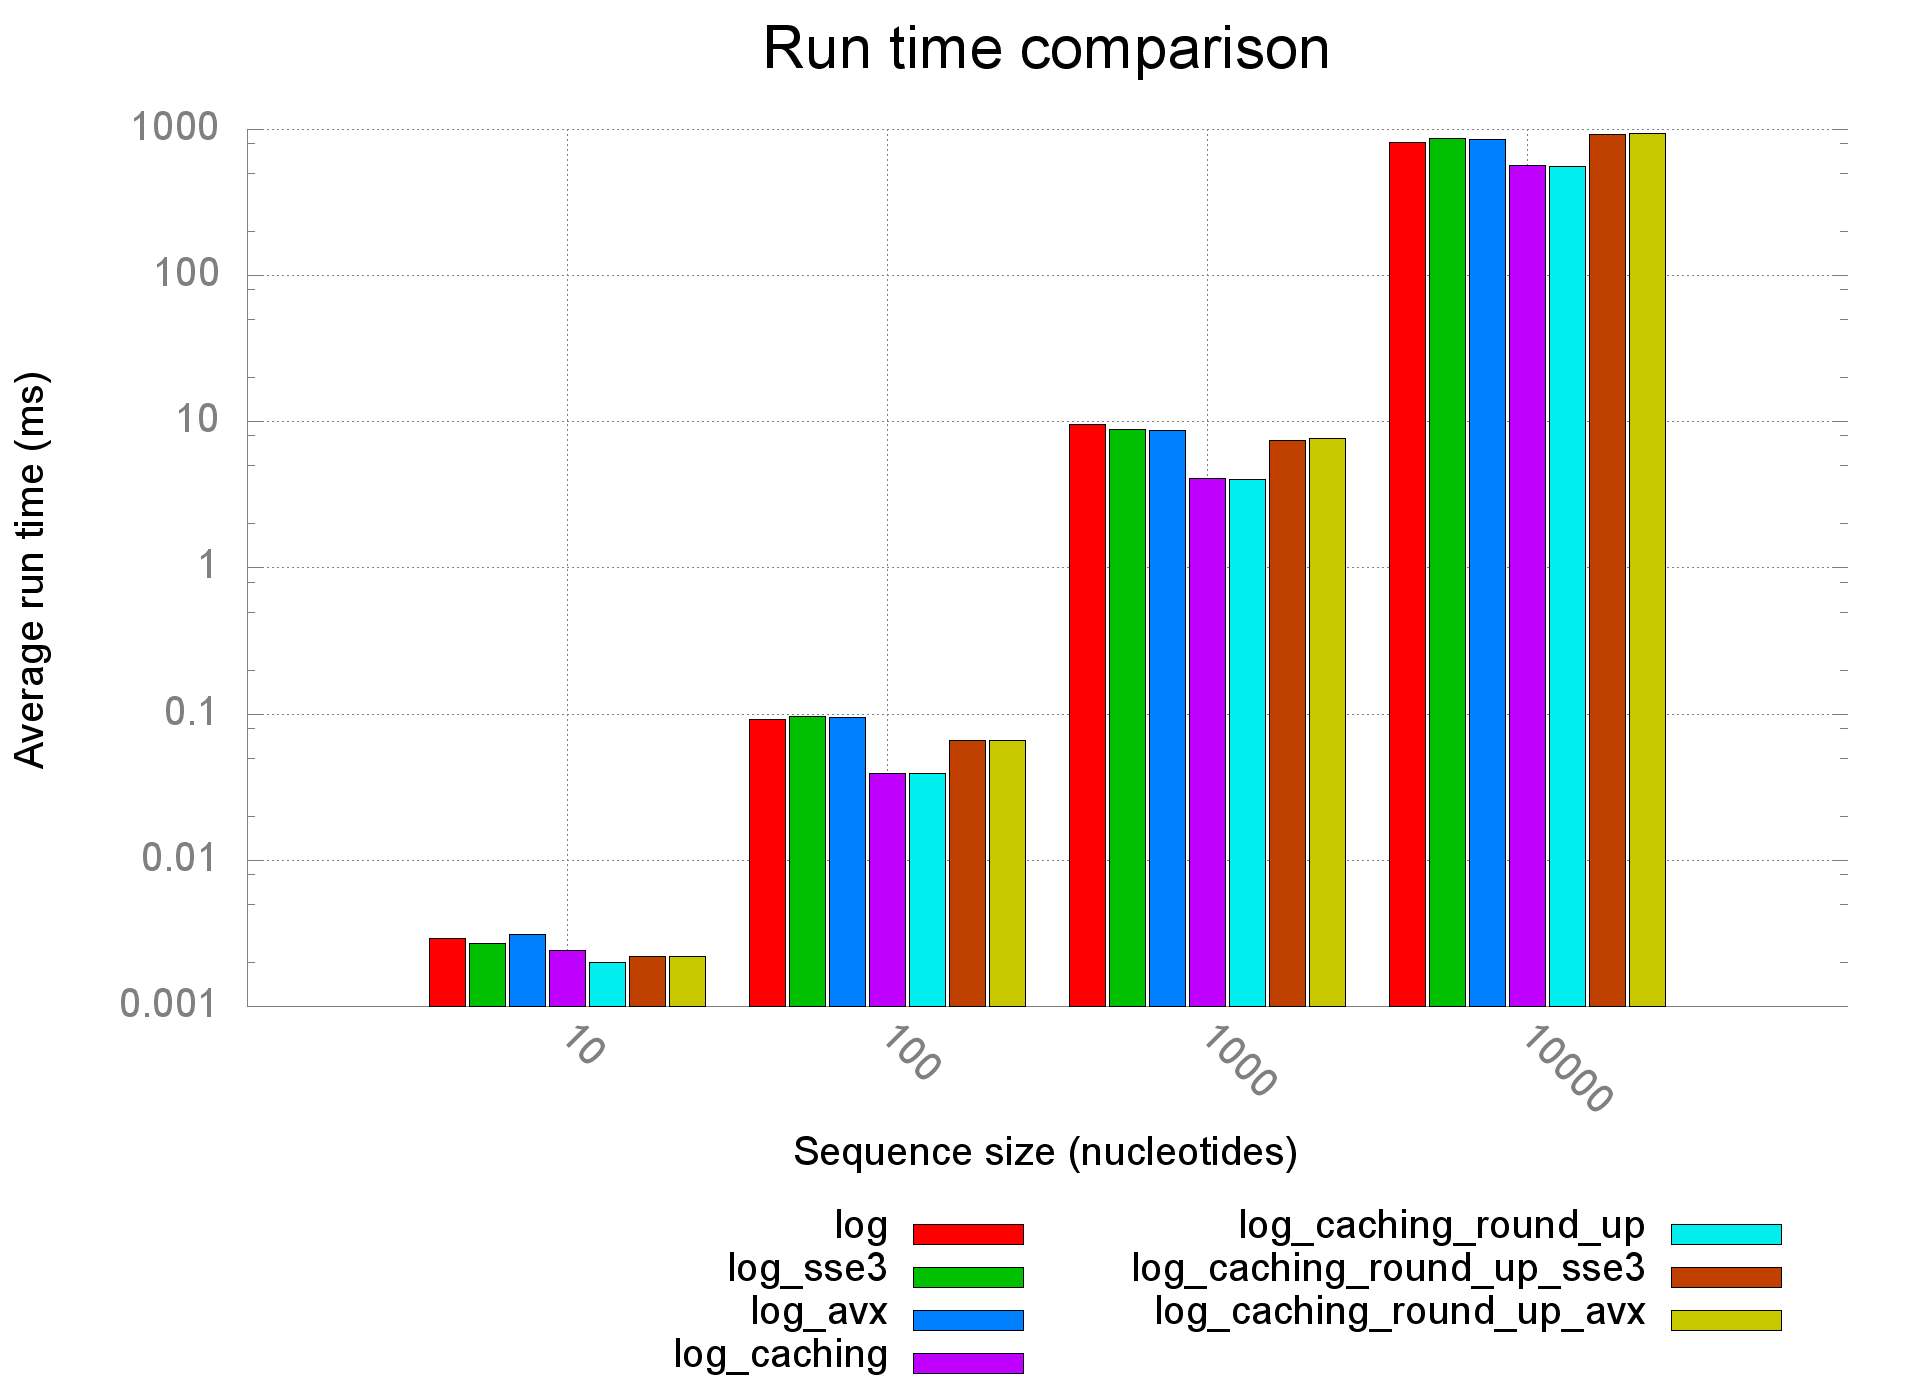
\includegraphics[width=\textwidth]{images/benchplot.png}
    \caption{Comparison of average runtimes of different implementations. \texttt{sse3} and \texttt{avx} post-fixes denote the vectorized versions of the programs,
using SSE3 and AVX vector intrinsics (Section~\ref{sec:vector}). With \texttt{log} we denote the log-space transformed versions of TKF91 (Section~\ref{sec:log}).
Versions using Arrays-of-Structs to store matrices (Section~\ref{sec:caching}) are denoted by \texttt{caching}; \texttt{round\_up} denotes versions relying on the \texttt{crlibm}
library logarithm function \texttt{log\_ru} (Section~\ref{sec:crlibm}).}
\label{fig:runtime}
\end{figure}



\begin{table}[]
\centering
\label{tbl:benchmark-teams}
\begin{tabular}{lll}
\begin{tabular}[c]{@{}l@{}}ms per iteration\\ (compared to best)\end{tabular}             & Team I                & Team II \\
BDNF                                                                                      & 83.1 (1.50)  & {\bf 55.4 (1.00)}  \\
cytb                                                                                      & 262.9 (1.25) & {\bf 209.9 (1.00)}  \\
RAG1                                                                                      & 209.1 (1.42) & {\bf 147.3 (1.00)} \\
RAG2                                                                                      & 246.1 (1.28) & {\bf 192.0 (1.00)}  \\
RBP3                                                                                      & 346.9 (1.25) & {\bf 277.6 (1.00)}  \\
vWF                                                                                       & 439.6 (1.25) & {\bf 352.2 (1.00)}
\end{tabular}
\caption{Performance comparison of TKF91 implementations by teams I \& II.}
\end{table}

\section{Teaching Results}
\label{teaching-results}
\subsection{What did Team I learn?}
While the assigned task was straightforward and very manageable in principle,
the implementation details were tricky.
Preventing floating point underflow while, at the same time, optimizing performance was challenging.
This is because, such technical problems are frequently ignored in other programming practicals at KIT
that focus on functionality.
Furthermore, vectorizing with SIMD intrinsics required some rethinking and re-engineering
because we needed to identify a suitable memory layout, optimize data alignment,
and deal with boundary conditions (padding).
While it was satisfying to address and solve problems progressively,
there were always additional ideas to further improve the code (w.r.t. performance and design),
which made prioritizing tasks important.
We enjoyed the satisfaction of gaining yet another percent of execution time in combination
with working with SIMD instructions that were not familiar to us.

The basic problem was clearly outlined. There was enough freedom and time left
to work on improving our solution. The scheduled project milestones
turned procrastination and last minute work into a non-issue.
Most surprisingly, we were always on schedule.



\subsection{What did Team II learn?}
For this assignment we had to tackle two major problems: preventing the loss of precision generated by numerical underflow {\bf SL: And why did we ignore other types of precision loss? We could have used compensated summation to become a little more correct. However, this could have decreased the overall speed} and
pursuing the elusive ``most efficient'' implementation.
In the early stages, we came up with the idea of transforming the algorithm into log-space to solve the numerical issues.
This did not only prove to represent an efficient solution, but also allowed us to further simplify the formulas and to pre-compute the vast majority of terms.
In this context we also discovered deviations in the output alignments
that depend on the specific implementation of the logarithm function being used.
We therefore used the \texttt{crlibm} library of mathematical functions, that allowed us to assess the impact of logarithm functions with distinct rounding strategies
on the final result.

To optimize the code we also used SSE3 and AVX intrinsics to vectorize the most work-intensive portions of the code.
While we were unable to produce a faster vectorized code, we did learn how to use vector intrinsics and how to deal with the associated pitfalls.
The largest performance gain was attained via a more cache-efficient data structure.
For this, we used profiling tools such as \texttt{perf} and \texttt{clang} for the first time.
Finally,  we concluded that \texttt{C++} is appropriate for HPC projects, provided that, the problem and data-structures at hand are well understood.


\section{Conclusion}
\label{conclusion}
We have implemented and made available two independent, highly optimized open-source implementations of the TKF91 algorithm for statistical pair-wise sequence alignment.
We thoroughly assessed their performance and investigated aspects such as differing alignment results because of slight numerical deviations in logarithm implementations.
The implementations by teams I and II are substantially different in the approach they take for optimizing program performance on standard x86 architectures.
We proposed several methods for storing and addressing the three dynamic programming matrices. In addition, we show how the original equations can be simplified
to (i) avoid numerical underflow issues and (ii) save a substantial amount of computations.

We make the source code available in the hope that, it will be useful to the community.
In particular, some of the wave-front vectorization approaches might be applied to the more complex statistical alignment kernels used in programs
such as BaliPhy~\cite{suchard2006bali}.

Finally, the task and code at hand can be used to design similar bioinformatics programming practicals. For instance, one might ask students to try and
come up with a faster implementation or use the existing implementations as library functions in some larger and more complex programming project.





%In this documentation we presented our implementation of the TKF91 evolutionary model for aligning sequences of DNA. Therefore we outlined the definition of an efficient memory layout, as well as measures to factor out complex computations during the tight loop in the DP algorithm. We presented our approach to the vectorization of the algorithm using SSE3 and AVX vector intrinsics and discussed how data can be efficiently aligned. Finally, the performance of the resulting application was tested and evaluated.

%As a final note, we would like to remark that keeping the data spatially coherent by adjusting the memory layout through interleaving the matrices did not result in the performance gain that had first been anticipated. Unfortunately, the penalty of the shuffling and blending during loading and storing vectors, which has been introduced by those memory layouts, almost perfectly outweighed the gain in cache locality, which can be seen in Table~\ref{tbl:benchmark-layout} in Section~\ref{sec:evaluation}.

\bibliographystyle{plain}
\bibliography{mlalign}

\end{document}
